\section{평가}\label{sec:eval}

평가는 네 개의 연구 질문에 답하는 형태로 구성한다.
\textbf{RQ1}: 절제 전체에서 각 요인의 효과 크기와 서열은 어떠하며,
III장의 진단(병목은 페치가 아니라 0-피연산자 데이터 이동)과
정합하는가.
\textbf{RQ2}: IV장의 세 원리 각각의 기여를 개발 이력의
준절제(quasi-ablation)로 분리할 수 있는가.
\textbf{RQ3}: 1차 비용 모델(식~\ref{eq:costmodel})은 레이어 간
이득 비대칭을 정합적으로 분해하는가.
\textbf{RQ4}: 표준 런타임(TFLM) 위의 통합은 얼마의 대가를 요구하는가.

실험 환경은 III장의 하네스와 동일하다: STM32F746G-DISCO(Cortex-M7
200MHz, I/D 캐시 각 4KB, RAM 총 320KB(DTCM 64KB 포함), 별도
ITCM-RAM 16KB)\cite{st_rm0385}, GNU Arm GCC 14.3.1, -O3+LTO. 절제
변형 A0--A4는 빌드 옵션으로 생성되며 A0는 기존 코드 경로와 메모리
레이아웃을 그대로 재현한다.

\subsection{RQ1: 절제 실측과 병목의 확증}

\begin{table*}[t]
\centering
\caption{누적 절제 실측(이미지당 ms, $T=30$, 동일 -O3+LTO 빌드).
모든 변형의 출력 스파이크 체크섬이 비트 일치한다.}
\label{tab:ablation}
\footnotesize
\setlength{\tabcolsep}{4.5pt}
\begin{tabular}{l l r r r r r r l}
\hline
변형 & 추가 적용 & total & 배율 & 인코딩 & CPL1 & CPL2 & FC$+$기타 & \texttt{FLASH\_ACR} \\
\hline
A0 & (기존 조건 재현) & 2,328.5 & 1.00$\times$ & 35.4 & 446.0 & 1,828.0 & 19.1 & 0x006 \\
A1 & $+$ART/프리페치 & 2,328.9 & 1.00$\times$ & 35.4 & 445.5 & 1,829.0 & 19.0 & 0x306 \\
A2 & $+$핫 커널 ITCM-RAM & 2,331.2 & 1.00$\times$ & 37.1 & 451.1 & 1,824.7 & 18.4 & 0x306 \\
A3 & $+$데이터 DTCM/SRAM & 2,178.7 & 1.07$\times$ & 37.1 & 401.8 & 1,719.8 & 20.0 & 0x306 \\
A4 & $+$이벤트 커널(제안) & \textbf{380.6} & \textbf{6.12$\times$} & 5.9 & 222.1 & 132.2 & 20.4 & 0x306 \\
\hline
\multicolumn{2}{l}{(참고) A4$'$: 동일 최적화의 비TFLM 직접 경로} &
372.8 & 6.25$\times$ & 6.1 & -- & -- & -- & 0x306 \\
\hline
\end{tabular}
\begin{flushleft}
\footnotesize 주: (a) ``FC$+$기타''는 total에서 인코딩$\cdot$CPL1$\cdot$
CPL2를 뺀 잔여(FC, TFLM 디스패치, 입력 복사 약 1.9ms, LIF\_out 포함).
각 셀은 원시 사이클에서 환산$\cdot$반올림한 값이다.
(b) \texttt{FLASH\_ACR}은 측정 당시 레지스터 실측값(0x306 $=$
ARTEN$|$PRFTEN$|$6WS) --- 각 변형의 조건 증명이다.
\texttt{SCB\_CCR}은 전 변형 0x70200(I/D 캐시$\cdot$분기예측 활성)으로
동일하며, ITCM 적재 바이트는 0/0/4,392/4,344/4,936B다. (c) A4$'$의 레이어
분해 계측점은 TFLM 경로 전용이라 표기하지 않는다. (d) 인코딩
개선(임계값 LUT 캐시, 비트 불변)은 A4에 포함된다.
\end{flushleft}
\end{table*}

표~\ref{tab:ablation}와 그림~\ref{fig:ablation}가 전체 결과다.
페치 계열(A1, A2)은 실질 무효과($\le$0.12\%), 데이터 재배치(A3)는
$+$7\%, 이벤트 커널(A4)은 A3 대비 단독 5.7배$\cdot$기준 대비
\textbf{6.12배}다. 효과의 서열 --- 페치 $0$, 배치 소폭, 트래픽 제거
지배 --- 는 III장의 진단과 일치한다. 특히 A1$\cdot$A2의
무효과는 그 자체로 보고 가치가 있는 부정적 결과다: 같은 두 최적화가
마이크로벤치마크에서는 각각 1.4배 이상$\cdot$최대 2.5배였다.

\begin{figure}[htbp]
\centering
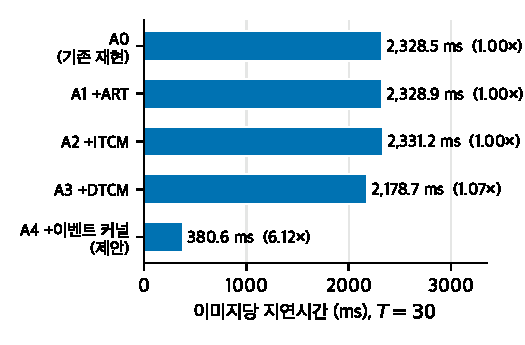
\includegraphics[width=0.92\linewidth]{figures/fig_ablation.pdf}
\caption{누적 절제별 이미지당 지연시간. 페치 계열(A1$\cdot$A2)은
무효과이고, 이득은 데이터 트래픽을 제거하는 이벤트 커널(A4)에
집중된다.}
\label{fig:ablation}
\end{figure}

\subsection{RQ2: 원리별 기여의 분해}\label{sec:rq2}

제안 커널은 한 번에 완성되지 않았다. 원리를 하나씩 실리콘에서
검증하며 다섯 차례 반복했고(그림~\ref{fig:iter}), 이 이력은 원리별
준절제에 해당한다 --- 단 k1에는 원리 2의 요소(2채널 레지스터
블로킹)가 일부 선반영되어 있고, 원리 3의 기여는 속도가 아니라 전
과정 무위반의 정확성 불변식이다. 전 과정에서 출력 체크섬은 한 번도
어긋나지 않았다(P3의 상시 감시).

\textbf{항등식 단독(k1, $2{,}178.7\rightarrow579.2$ms)}: 이벤트
목록을 im2col 컬럼에서 만들고 조밀 레이아웃 가중치를 2채널씩
gather하는 최소 구현만으로 3.8배 --- 식~(\ref{eq:collapse})의 이득이
지배적임이 실증된다. \textbf{P1 완성(k2, $\rightarrow504.3$ms)}:
값 실체화를 제거하고 수용 영역에서 위치를 직접 스캔하자 74.9ms가
추가로 사라졌다 --- im2col 트래픽의 소멸분이다.
\textbf{P2 전반(k3, $\rightarrow457.5$ms)}: 가중치 전치는 예측대로
CPL2를 $249.5\rightarrow148.4$ms로 개선했으나, CPL1은
$228.7\rightarrow282.8$ms로 \textbf{퇴행}했다. CPL1 가중치는 이미
DTCM 상주라 지역성 개선의 여지가 없는데, 이 버전이 누산기를 메모리
배열에 두어 원소당 적재-가산-저장이 추가된 탓이다.
\textbf{P2 후반(k4, $\rightarrow382.2$ms)}: 8채널 레지스터 블로킹이
퇴행을 회복시키며(CPL1 $223.2$ms) CPL2도 추가
개선($132.9$ms)했다. 지역성과 레지스터 상주가 \emph{함께여야}
원리가 성립함을 퇴행-회복 쌍이 보여준다. \textbf{P1의 밀도
적응(k5, $\rightarrow380.6$ms)}: 고밀도 레이어의 무분기 스캔은
1.0ms 개선에 그쳤다 --- 컴파일러가 이미 조건부 실행을 생성하고
있었던 것으로 보이며, 기각된 가설로 기록한다. 측정 출처를
명확히 하면, k1--k4는 하네스 정비(III장) \emph{전}의 개발
기록이고(정비로 제거된 노이즈는 0.2\% 미만) 표~\ref{tab:ablation}의
A계열과 k5는 정비 후 재측정값이다.

\begin{figure}[htbp]
\centering
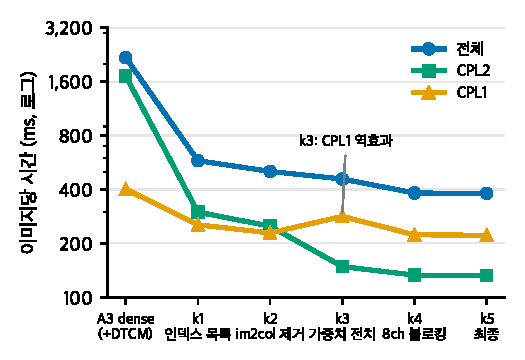
\includegraphics[width=0.95\linewidth]{figures/fig_kernel_iter.pdf}
\caption{원리별 검증의 이력(로그 축). k3의 CPL1 퇴행과 k4의 회복이
원리 2의 두 요소(지역성$\cdot$레지스터 상주)가 각각 필요함을
보인다.}
\label{fig:iter}
\end{figure}

\subsection{RQ3: 레이어 비대칭과 비용 모델}\label{sec:rq3}

그림~\ref{fig:layers}의 레이어 분해가 보이듯, 같은 커널의 이득은
발화 밀도에 따라 크게 갈린다: 밀도 4.1\%의 CPL2는
$1{,}719.8\rightarrow132.2$ms(13.0배), 밀도 47.7\%의 CPL1은
$401.8\rightarrow222.1$ms(1.8배)다. 시간비로는 각각 0.077과
0.553이고, 식~(\ref{eq:costmodel})에 대입하면 $\alpha\approx0.032$,
$\beta\approx1.09$를 얻는다. 두 점으로 두 파라미터를 정하는 것이므로
이는 검증이 아니라 \emph{분해}다. 모델의 내용은 해석에 있다:
$\beta\approx1.09$는 이벤트 1개의 처리 비용(인덱스 적재$+$8채널
가산)이 조밀 원소 1개의 비용(SMLALD MAC$+$피연산자 적재)과 거의
같다는 뜻이고, 따라서 이득은 거의 전적으로 ``건너뛴 원소 수''에서
나온다. $\alpha\approx0.032$는 스캔$\cdot$에필로그의 고정 몫으로,
이 커널 형상의 이득 상한이 약 $1/\alpha\approx31$배임을 말한다 ---
CPL2의 13.0배는 상한의 42\% 지점이다. 모델의 외삽적 함의는 VI장에서
다룬다.

\begin{figure}[htbp]
\centering
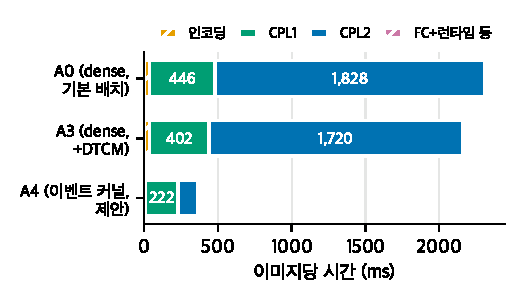
\includegraphics[width=0.95\linewidth]{figures/fig_layers.pdf}
\caption{레이어 분해. 동일 커널의 이득이 발화 밀도에 따라
13.0$\times$(CPL2, 4.1\%)와 1.8$\times$(CPL1, 47.7\%)로 갈린다 ---
병목이 CPL2에서 CPL1로 이동한다.}
\label{fig:layers}
\end{figure}

\subsection{RQ4: 표준 런타임의 대가}

동일 최적화를 적용한 비TFLM 직접 경로 A4$'$는 372.8ms로, 런타임의
대가는 이미지당 7.8ms(2.1\%)다. $T{=}30$회의 Invoke 반복에도
해석기 기반 런타임이 수용 가능한 비용에 머문다는 선행 연구의
결론\cite{cha2026fusion}은 추론이 6배 빨라진 뒤에도 유지된다.
부수적으로, 두 경로는 LIF1 스파이크 진폭이 다름에도(직접 경로
$S_1{=}16{,}384$, TFLM 경로 $32{,}767$ --- 배율은 requantize 계수에
흡수) 출력 체크섬까지 일치했다 --- 계약(4.1절)이 구현 변형에
강건함을 보이는 독립 증거다.

\subsection{계약의 검증}\label{sec:checksum}

회귀 판정은 출력 스파이크 체크섬 --- 매 타임스텝 10개 출력 스파이크
값의 부호 없는 16비트 누적 합(8장$\times$30스텝$\times$10출력,
$2{,}400$개 값) --- 으로 한다. LIF는 막전위가 30스텝에 걸쳐 누적되는
상태 기계이므로 네트워크 어디서든 1 LSB의 차이가 발화 타이밍
연쇄로 증폭된다: 체크섬은 단순하지만 민감하다. 실측 결과
\textbf{A0--A4와 A4$'$, 여섯 빌드의 체크섬이 전부
동일}(0x00E9FE2C)했고 8장의 예측도 전부 일치했다(7/8 정답; 표본
8장은 데모 규모로 정확도 지표가 아니다). 한계도 명시한다: 단순
합이라 오류의 상쇄 우연이 이론상 가능하고 검증 범위는
8장$\times$30스텝이 실행한 경로다. 전자는 예측 일치가, 후자는
4.1절의 구성적 논증이 보완하며, dense 경로 자체의 정당성은 선행
연구의 호스트 검증(LIF SIMD $1{,}887$만 조합 전수 비교
포함)\cite{cha2026fusion}이 담보한다.

\subsection{자원 사용}

최종 빌드(A4)의 정적 사용량은 RAM $283{,}072$B(전치 가중치 사본
154KB와 아레나 64KB 설정 포함), Flash $296{,}432$B이다. TCM 사용은
표~\ref{tab:placement}과 같고(DTCM 89\%, ITCM 30\%), LIF
상태$\cdot$스크래치가 아레나 밖으로 나가면서 TFLM 아레나 실사용은
$79{,}764$B에서 $25{,}940$B로 줄었다. 예산은 링크 타임 ASSERT로
강제된다.
